\documentclass[aspectratio=169, t, 8pt]{beamer}

%------configurando acentos-----------
\usepackage[utf8]{inputenc}
\usepackage[brazil]{babel}

\usepackage{graphicx}

%-------Estilos Beamer---------------
\usetheme{metropolis}
%\usecolortheme{crane}
%coment
%\usefonttheme{serif}
\linespread{1.2}

% Personalização de Cores (Exemplo: Minimal Teal)
% Cores Base
\definecolor{BgCanvas}{HTML}{F9F9FB}      % Off-white muito suave
\definecolor{MainText}{HTML}{2B2D42}      % Grafite escuro para alta legibilidade
\definecolor{PrimaryAccent}{HTML}{4A6FA5} % Az
\definecolor{SunCoastFg}{HTML}{F2A154}
% --- CONFIGURAÇÕES DE TEMA BEAMER ---
%\usetheme{metropolis}

\setbeamertemplate{itemize item}{\textcolor{MainText}{$\bullet$}}
\setbeamertemplate{itemize subitem}{\textcolor{MainText}{\scriptsize$\circ$}}
\setbeamertemplate{itemize 3rditem}{\textcolor{MainText}{\tiny$\blacksquare$}}

\setbeamercolor{background canvas}{bg=BgCanvas}
\setbeamercolor{normal text}{fg=MainText}
\setbeamercolor{frametitle}{bg=SunCoastFg, fg=BgCanvas}
\setbeamercolor{title}{fg=MainText}
\setbeamercolor{subtitle}{fg=PrimaryAccent}
\setbeamercolor{structure}{fg=PrimaryAccent}

% Remove a linha amarela padrão do Metropolis sob o título
\setbeamertemplate{title separator}{}
\setbeamertemplate{progress bar in section page}{}


%--------Dados do Documento
\title{Matemática: Lista de Exercícios}
\author{prof. Eduardo}
\institute{Pré-Universitário Oficina do Saber / UFF}
\date{\today}


%-------- Pacotes Matemática -------------
\usepackage{amsmath}
\usepackage{amsthm}
\usepackage{amsfonts}
\usepackage{amssymb}
\usepackage{xfrac}
\usepackage{thmtools}

%-------- Configuração Listas---------
% \usepackage{enumitem}
\usepackage[inline]{enumitem}

\setcounter{tocdepth}{2}

\newcounter{questaovest}
\newcommand{\vest}[1]{\stepcounter{questaovest}\item[\textbf{Questão \arabic{questaovest}} (#1):]}
\setlist[enumerate]{
    align=left,
    leftmargin=1.8em,
    itemindent=1.8em
    }

\setlist[enumerate,2]{
    label=\alph*.,
    font=\bfseries,
    itemsep=0.1pt,
    labelsep=0em,
    parsep=0pt,
    leftmargin=0em,
    }

%------------- Atalho para imagens ------------
\graphicspath{{../../src/img/semana06/}}


\begin{document}

\begin{frame} %capa
        \vspace*{\fill}
            
            \begin{columns}[c]
                \begin{column}{0.5\textwidth}
                    {\usebeamerfont{title}\usebeamercolor[fg]{title}\inserttitle}\vspace{0.2cm}
                    
                    {\usebeamerfont{subtitle}\usebeamercolor[fg]{subtitle}\insertsubtitle}\vspace{0.5cm}

                {\usebeamerfont{author}\insertauthor}\vspace{0.3cm}

                {\usebeamerfont{institute}\insertinstitute}\vspace{0.3cm}

                {\usebeamerfont{date}\insertdate}
            \end{column}
            
            
            \begin{column}{0.4\textwidth}
                \centering
                
\includegraphics[width=0.4\textwidth]{../logo_ofSaber.png}

                \vspace{.4cm}
                \vspace*{\fill}
        \begin{columns}[c]
            \begin{column}{.5\textwidth}
                \centering
\includegraphics[width=.5\textwidth]{../Proex02c.png}
            \end{column}
            \begin{column}{.5\textwidth}
                \centering
\includegraphics[width=0.4\textwidth]{../Logo_UFF.png}
            \end{column}
        \end{columns}
        \vspace*{\fill}
            \end{column}
        \end{columns}
    \vspace*{\fill}
    \end{frame}
    
        % {
        %     \usebackgroundtemplate{
        %     
\includegraphics[width=\paperwidth]{slide_02_contracapa.png}}
        %     \begin{frame}[plain]                
        %     \end{frame}
        % }


    \begin{frame} %Questão 01-B
        \frametitle{Combinatória}
        \vspace{-1.2em}
        \begin{enumerate}
            \begin{columns}
                \begin{column}{.9\textwidth}
                    \vest{ENEM-2015} Um cliente de uma videolocadora tem o hábito de alugar dois filmes por vez. quando os devolve, sempre pega outros dois filmes e assim sucessivamente. Ele soube que a videolocadora recebeu alguns lançamentos, sendo 8 filmes de ação, 5 de comédia e 3 de drama e, por isso, estabeleceu uma estratégia para ver todos esses 16 lançamentos. Inicialmente alugará, em cada vez, um filme de ação e um de comédia.

                    Quando se esgotarem as possibilidade de comédia, o cliente alugará um filme de ação e um de drama, até que todos os lançamentos sejam vistos e sem que nenhum filme seja repetido.

                    De quantas formas distintas a estratégia desse cliente poderá ser posta em prática?

                    \vspace{1em}
                            \raggedleft
                            \begin{minipage}{\textwidth}
                                \begin{enumerate*}[itemjoin={\hfill}]
                                    \item $20 \times 8! + (3)^2$
                                    \item $8! \times 5! \times 3!$
                                    \item $\displaystyle\frac{8! \times 5! \times 3!}{2^8}$
                                    \item $\displaystyle\frac{8! \times 5! \times 3!}{2^2}$
                                    \item $\displaystyle \frac{16!}{2^8}$
                                    %gabarito: B
                                \end{enumerate*}
                            \end{minipage}

                \end{column}
            \end{columns}
        \end{enumerate}
    \end{frame}

    \begin{frame} %Questão 02-E
        \frametitle{Geometria}
        \begin{columns}
            \begin{column}{.9\textwidth}
                \begin{enumerate}
                    \vest{ENEM-2018} O remo de assento deslizante é um esporte que faz uso de um barco e dois remos do mesmo tamanho. A figura mostra uma das posições de uma técnica chamada afastamento.

                    Nessa posição, os dois remos se encontram no ponto $A$ e suas outras extremidades estão indicadas pelos pontos $B$ e $C$. Esses três pontos formam um triângulo $ABC$ cujo ângulo $\widehat{BAC}$ tem medida de $170^\circ$.

                    O tipo de triângulo com vértices nos pontos $A, B$ e $C$, no momento em que o remador está nessa posição, é
                    \vspace{1.2em}
                    \begin{columns}[T, totalwidth=.8\textwidth]
                        \begin{column}{.45\textwidth}
                            \begin{figure}
                                \centering
                                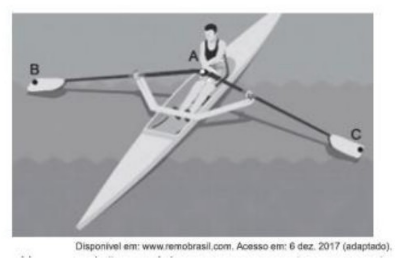
\includegraphics[width=0.9\textwidth]{monitoria_questao02.png}
                            \end{figure}
                        \end{column}
                        \begin{column}{.35\textwidth}
                            \begin{enumerate}
                                \item retângulo escaleno
                                \item acutângulo escaleno
                                \item acutângulo isósceles
                                \item obtusângulo escaleno
                                \item obtusângulo isósceles
                            \end{enumerate}
                        \end{column}
                    \end{columns}
                \end{enumerate}
            \end{column}
        \end{columns}
    \end{frame}

    \begin{frame} %Questão 03-A
        \frametitle{Volume}
        \begin{columns}[T, totalwidth=.9\textwidth]
            \begin{column}{\textwidth}
                \begin{enumerate}
                    \vest{ENEM-2017} Para as Olimpíadas de 2012, a piscina principal do Centro Aquático de Londres, medindo 50 metros de comprimento, foi remodelada para ajudar os atletas a melhorar suas marcas. Observe duas das melhorias:
                    \begin{columns}[T, totalwidth=.9\textwidth]
                        \begin{column}{.6\textwidth}
                            \centering
                            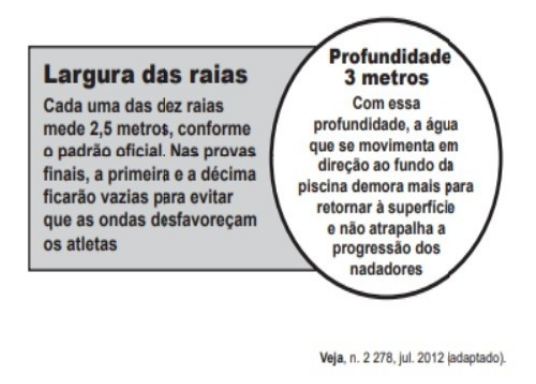
\includegraphics[width=\textwidth]{monitoria_questao03.png}
                        \end{column}
                        \begin{column}{.35\textwidth}
                            A capacidade da piscina em destaque, em metro cúbico, é igual a
                            \begin{enumerate}
                                \item 3750
                                \item 1500
                                \item 1250
                                \item 375
                                \item 150
                            \end{enumerate}
                        \end{column}
                    \end{columns}
                \end{enumerate}
            \end{column}
        \end{columns}
    \end{frame}
    
    \begin{frame} %Questão 04-B
        \frametitle{Geometria}
        \begin{columns}[T, totalwidth=.9\textwidth]
            \begin{column}{\textwidth}
                \begin{enumerate}
                    \vest{ESPM-2018} O número de anagramas da palavra \textbf{COLEGA} em que as letras L, E e G aparecem juntas em qualquer ordem é igual a:
                    
                    \vspace{1.6em}

                    \centering
                    \begin{minipage}{.8\textwidth}
                        \begin{enumerate*}[itemjoin={\hfill}]
                                \item 72
                                \item 144
                                \item 120
                                \item 60
                                \item 24
                    \end{enumerate*}
                    \end{minipage}
                \end{enumerate}
            \end{column}
        \end{columns}
    \end{frame}

    \begin{frame} %Questão 05-A
        \frametitle{Geometria}
        \begin{columns}[T, totalwidth=.9\textwidth]
            \begin{column}{\textwidth}
                \begin{enumerate}
                    \vest{ENEM-2017} Suponha que para um trem trafegar de uma cidade à outra seja necessária a construção de um túnel com altura e largura iguais a $10$m. Por questões relacionadas ao tipo de solo a ser escavado, o túnel deverá ser tal que qualquer seção transversal seja o arco de uma determinada parábola, como apresentado na Figura 1.

                    Deseja-se saber qual a equação da parábola que contém esse arco. Considere um plano cartesiano com centro no ponto médio da base da abertura do túnel, conforme Figura 2.

                    A equação que descreve a parábola é:
                    \vspace{1em}
                    \begin{columns}[T, totalwidth=.9\textwidth]
                        \begin{column}{.3\textwidth}
                            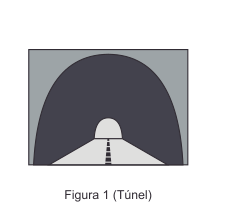
\includegraphics[width=\textwidth]{monitoria_questao05_1.png}
                        \end{column}
                        \begin{column}{.3\textwidth}
                            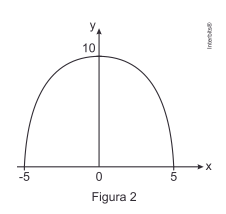
\includegraphics[width=\textwidth]{monitoria_questao05_2.png}
                        \end{column}
                        \begin{column}{.2\textwidth}
                            \begin{enumerate}
                                \item $\displaystyle y = - \frac{2}{5}x^2 +10$\vspace{0.5em}
                                \item $\displaystyle y = \frac{2}{5}x^2 +10$\vspace{0.5em}
                                \item $y=-x^2 +10$\vspace{0.5em}
                                \item $y=x^2 -25$\vspace{0.5em}
                                \item $y=-x^2+25$
                            \end{enumerate}
                        \end{column}
                    \end{columns}
                \end{enumerate}
            \end{column}
        \end{columns}
    \end{frame}

    % \begin{frame} %Questãao 06-B
    %     \frametitle{Geometria}
    %     \begin{columns}[T, totalwidth=.9\textwidth]
    %         \begin{column}{\textwidth}
    %             \begin{enumerate}
    %                 \vest{PUCR-RS/2013} Um desafio matemático construído pelos alunos do Curso de Matemática tem as peças no formato de um cone. A figura abaixo representa a planificação de uma das peças construídas.
    %                 \vspace{0.5em}
    %                 \begin{columns}[T, totalwidth=.9\textwidth]
    %                     \begin{column}{.4\textwidth}
    %                         \centering
    %                         
\includegraphics[width=.9\textwidth]{lista_q06.png}
    %                     \end{column}
    %                     \begin{column}{.4\textwidth}
    %                         A área total dessa peça é de \underline{\hspace{.5cm}} $\text{cm}^2$

    %                         \vspace{1em}
                            
    %                         \begin{enumerate*}[itemjoin={\hfill}]
    %                             \item $10\pi$
    %                             \item $16\pi$
    %                             \item $20\pi$
    %                             \item $28\pi$
    %                             \item $40\pi$
    %                             % gabarito B 
    %                         \end{enumerate*}
    %                     \end{column}
    %                 \end{columns}
    %             \end{enumerate}
    %         \end{column}
    %     \end{columns}
    % \end{frame}

\end{document}